\documentclass[12pt]{article}

\usepackage{geometry}
\geometry{a4paper, left=20mm, right=20mm, top=20mm, bottom=20mm}

\setlength{\parindent}{2em}
\setlength{\parskip}{1em}

\usepackage{hyperref}

\usepackage{syntonly}
%\syntaxonly
\usepackage{amsmath}
\usepackage{amssymb}

\usepackage[utf8]{inputenc}
\usepackage[backend=biber,style=numeric,sorting=none,]{biblatex}
\addbibresource{ref.bib}

\usepackage{graphicx}

% aliasis
% FreeSurfer from Havord Unv.
\newcommand{\FS}{\href{http://surfer.nmr.mgh.harvard.edu}{\textbf{FreeSurfer}}} 

% encoders
% vector or matrix
\newcommand{\vecEC}[1]{\boldsymbol{#1}}

% decoders
\newcommand{\vecDC}[1]{\boldsymbol{\tilde{#1}}}

\newcommand{\xVO}{\boldsymbol{x}}         % the x vector, original
\newcommand{\xVR}{\boldsymbol{\tilde{x}}} % the x vector, recovered
\newcommand{\xSO}{x}                      % the x scaler, original
\newcommand{\xSR}{\tilde{x}}              % the x scaler, recovered

% the eta vector
\newcommand{\etaEC}{\vecEC{\eta}}                % generic encoder
\newcommand{\etaEi}{\WEC_i^{d_{i+1} \times d_i}} % encoder layer i
\newcommand{\etaDC}{\vecDC{\eta}}                % generic decoder
\newcommand{\etaDi}{\WDC_i^{d_i \times d_{i+1}}} % decoder layer i

% the W matrix
\newcommand{\WEC}{\vecEC{W}}                   % generic encoder
\newcommand{\WEi}{\WEC_i^{d_{i+1} \times d_i}} % encoder layer i
\newcommand{\WEI}[3]{\WEC_{#1}^{d_{#2} \times d_{#3}}} % decoder layer #i
\newcommand{\WEIt}[3]{\WEC_{#1}^{d_{#2} \times d_{#3}\prime}} % decoder layer #i, transposed
\newcommand{\WDC}{\vecDC{W}}                   % generic decoder
\newcommand{\WDi}{\WDC_i^{d_i \times d_{i+1}}} % decoder layer #i
\newcommand{\WDI}[3]{\WDC_{#1}^{d_{#2} \times d_{#3}}} % decoder layer #i
\newcommand{\WDIt}[3]{\WDC_{#1}^{d_{#2} \times d_{#3}\prime}} % decoder layer #i

% the w vector
\newcommand{\wEC}{\vecEC{w}}    % generic encoder
\newcommand{\wEI}[2]{{\wEC_{#1}^{1 \times d_{#2}}}}
\newcommand{\wDC}{\vecDC{w}}    % generic decoder
\newcommand{\wDI}[2]{{\wDC_{#1}^{1 \times d_{#2}}}}
\newcommand{\wDIt}[2]{{\wDC_{#1}^{1 \times d_{#2}\prime}}}

% the b vector
\newcommand{\bEC}{\vecEC{b}}    % generic encoder
\newcommand{\bEi}{\bEC_i^{d_i}} % encoder layer i
\newcommand{\bEI}[2]{\bEC_{#1}^{d_{#2}}} % encoder layer i
\newcommand{\bDC}{\vecDC{b}}    % generic decoder
\newcommand{\bDi}{\bDC_i^{d_i}} % encoder layer i
\newcommand{\bDI}[2]{\bDC_{#1}^{d_{#2}}} % encoder layer i

% the x vector
\newcommand{\xEC}{\vecEC{x}}    % generic encoder
\newcommand{\xDC}{\vecDC{x}}    % generic decoder
% the X matrix
\newcommand{\XEC}{\vecEC{X}}    % generic encoder
\newcommand{\XDC}{\vecDC{X}}    % generic decoder

% the y_hat vector
\newcommand{\yHT}{\boldsymbol{\hat{y}}}
\newcommand{\YHT}{\boldsymbol{\hat{Y}}}

% the z vector
\newcommand{\zEC}{\vecEC{z}}    % generic encoder
\newcommand{\zDC}{\vecDC{z}}    % generic decoder

% I/O for decoder layer
\newcommand{\iDi}{\zDC_{i+1}^{d_{i+1}}}
\newcommand{\zEI}[2]{{\zEC_{#1}^{d_{#2}}}}
\newcommand{\zEIt}[2]{{\zEC_{#1}^{d_{#2}\prime}}}
\newcommand{\oDi}{\zDC_i^{d_i}}
\newcommand{\zDI}[2]{{\zDC_{#1}^{d_{#2}}}}
\newcommand{\zDIt}[2]{{\zDC_{#1}^{d_{#2}\prime}}}

% the vector of ones
\newcommand{\one}{\boldsymbol{1}}         % the z vector in encoders
% the diagnal matrix
\newcommand{\I}[1]{\boldsymbol{I}^{#1}}

% parameters in the neural network
\newcommand{\Par}{\boldsymbol{\Theta}} % the parameters
\newcommand{\pEC}{\boldsymbol{\theta}} % the parameters in the stacked autoencoder
\newcommand{\pDC}{\boldsymbol{\tilde{\theta}}} % the parameters in the decoder

% Loss function in Cross Entropy form
\newcommand{\LCE}[2]{#1\log{#2} + (1 - #1)\log{(1 - #2)}}

% derivative
\newcommand{\DRV}[2]{\frac{d #1}{d #2}}        % derivative
\newcommand{\DRC}[3]{\DRV{#1}{#2}\DRV{#2}{#3}} % chained derivative
\newcommand{\PDV}[2]{\frac{\partial #1}{\partial #2}} % paritial derivative
\newcommand{\PDC}[3]{\PDV{#1}{#2}\PDV{#2}{#3}}        % chained

% invers logit, aka. sigmoid function
\newcommand{\SGM}[1]{\frac{1}{1+e^{-#1}}}

% assign to diagnoral
\newcommand{\diag}[1]{\text{diag}(#1)}

\pagestyle{headings}

\author{Xiaoran Tong}

\begin{document}
\title{An Joint Association Analysis Method for Genomic Sequencing and Neuroimaging Data}
\maketitle

\begin{abstract}
The next generation genome sequencing and medical imaging technology give rise to large, mult-site cohort with growing wealth of next generation sequencing (NGS) and imaging profiles, which mandates the development of analytical methods capable of utilizing both type of information to identify predictive biomarkers of disorders. However, we are met with “the curse of dimensionality and multiple testing”, due to the large number of variants in these profiles. In this study, we try to tackled the dimensionality issue by sending the 3 dimensional cortical surfaces through stacked audoencoders constructed by unsupervised machine learning technique, which produce compact high order feature of the original surface, following which a similarity based U statistic were used to evaluate the joint association of the high order image features, the genome profile, and the phenotype of interest.
We conducted simulation studies and real data analysis using the deep genomic sequencing and neuroimage data provided by the Alzheimer’s Disease Neuroimaging Initiative (ADNI). The study demonstrated higher power with the joint analysis than either genome or image data alone, also demonstrated is the power improvement achieved by replace raw images with high order features abstracted from them. 
\end{abstract}

\section{Introduction}
The decade long search of casual variant by genome wide association analysis (GWA) hasn't been satisfying. So far GWA hardly find any single nucleotide variant (SNV) with an large enough effect to act as a stand along necessary cause of any complex diseases. Although a large number of statistically significant common variants were indeed identified by GWA, only a moderate fraction of heritability have been explained by the totality of these finding\cite{GWA1, GWA2}. Despite the setback, human genome is still an intriguing source of curiosity owning to its intrinsic advantages. When viewed as an exposure, genetic polymorphism is constant throughout an individual's life course and all types of organism, saving the complication of study design. Also, as one of the fundamental causes of all biological processes, genomic polymorphism is not susceptible to reverse causality. From a population perspective, the occurrence of genetic variation mimic a random assignment of treatment in an quasi-experiment, which in turn can be exploited to infer non-genetic effect through an instrumental variable approach, such as Mendelian Randomization \cite{MR1, MR2}. These features keeps genomic analysis a promising tool for casual inference.

\subsection{Analysis of Rare Genomic Variants}
The "rare variant, common disease (RVCD)" hypothesis aims to to explain of the "missing heritability" which GWA failed to capture. RVCD states the gap could be attributed to rare variants of moderate to large effect not covered by GWA \cite{RVCD1}. The Next Generation Sequencing (NGS) projects, growing in both number and scale over the last decade, offered numerous data sources for the analysis of rare variants. However, the stockpiling data also raise a number of methodological challenges. For one, the variants in a NGS profile is much denser than a GWA profile, which poses intense computation and multiple testing should the traditional per-variant based screening procedures is applied. Also, as the name suggested, the newly detected rare variants came with their minor allele frequencies (MAF) close to 0. As a consequence, the lack of heterogeneity in genotype threatens the statistical power for studies of moderate and small sample size. So far the most popular remedy is signal aggregation, that is, instead of screening the whole profile one variant after another, we first group the variants according to certain criteria, and subsequently all the variants in one group are tested together as an unit, during which the signal of the members are aggregated. The aggregation can be achieved by either collapsing the grouped variants into a single variant \cite{Burden1} before the statistical test, or by testing all the variants together with a multivariate approach \cite{UST1, UST2, SKT}. The aggregation can also be done after a per-variant screening, by summarizing the test statistics (e.g. p-values) of group members into one statistics \cite{Dai:2015, plink1}. Grouping and aggregation drastically reduce the number of hypothesis testing, and improve the heterogeneity or the testing unit. A dilemma comes along though, is the choice of grouping criteria. The most common criteria refer prior knowledge of biological function, resulting in gene or pathway based grouping. One could also group the variants by every few or by a threshold of linkage disequilibrium (LD) \cite{plink1}. Since the focus of this study is hypothesis testing, for now, we adopt a gene based grouping scheme for both simulation and real data analysis.

\subsection{Incorporating Imaging Data}
A hard truth contributing to the unsatisfactory performance of GWA is the genetic effect being intrinsically weak over a complex disease, owning to the large ``black box'' between the upstream genomic variants and the health outcome at the downstream far end. It is always desirable to probe the ``black box'' by incorporating other intermediate biological profiles. The added information should increase the chance of detecting strong association, especially when the new profiles is in the casual pathway from the genomic profile to the disease. Our method borrows additional information from neroimaging data, knowing that the cerebral structure is a powerful indicator of neurological disorder. Much like the GWA, similar, per-variant screening procedures can be applied to image profiles if proper definition of variants and their values are given. Taking the structured MRI as an example, it is natural to view voxels in the MRI slices as variants, and the normalized brightness of those voxels as their values. Following such definition, a per-voxel screening can be immediately done to the entire profile to search for significant loci in the brain, which is typically called voxel-wise analysis (VWA) \cite{VWA1, VWA2, VWA3, VWA4}. In our study, the neuroimaging profiles are processed by \FS, a freely distributed neuroimaging processing software. Instead of the original structure MRI slices, the cortex reconstructed from these slices is taken as image profile. Instead of the voxels, the variants are redefined as the vertices spanning the 3D cortex, while the values are defined as the gray matter thickness at these vertices. \FS already comes with its own vertex-wise analysis (the abbreviation happens to be ``VWA'' as well), which in essential is applying generalized mixed linear model to very vertex \cite{FS:Anl1, FS:Anl2}. The per-variant screening approach may work better for the cortex than for the genomic profile, because the value of an vertex is continuous, which mean it does not suffer low variability like a rare genomic variant does. However, the multiple testing issue might be worsen because the neighboring image variants cover tightly connected cerebral tissue, their value (thickness of gray matter) are highly correlated. Thus, the grouping and aggregation strategy could also benefit analysis involving cortex profiles. As an analogy of gene based grouping and aggregation of genomic variants, the cortical vertices can be conveniently grouped into 68 recognized functional anatomy regions (34 in each hemisphere) and have each of them analyzed as an unit. In the simulation study, we will take out small regions from the cortex and compare the power performance of an aggregated unit against the per-variant based VWA.

\subsection{Dimension reduction using Deep Artificial Neural Network}
The typical testing unit of the image profile is also high dimensional, oftentimes even higher then most of the genomic testing units. For our study data, after segregating cortex into 68 anatomy regions with \FS, the chance of a randomly picked cortex region holding more variants than a randomly picked gene is 96.8\%. Although the multivariate algorithms that works with genomic testing unit can be applied to the cortex with little to no rework, it would be desirable to first reduce the dimensionality of a image based test unit before the analysis. One popular trend is using deep artificial neural network to extract high order features from the raw profile, which not only lowers the dimensionality but also raises the signal - noise ratio \cite{DL:Intro1}. The potent of deep network lies in its capability to cumulatively encrypt incoming knowledge with unsupervised training technique. In other words, as long as the future collection of image data follows protocols compatible to the current, the existing deep network can be incrementally refined to achieve more precise and concise feature abstraction. For now, included in the method is a series of stacked autoencoders for each the cortical regions, which are light weighted deep network whose capability is comparable to the more powerful but much slower deep belief networks \cite{DL:SDA1, DL:Intro2}. The formulation and calibration of the stacked autoencoder is detailed in the method section and appendix, simulation studies are conducted to compare the performance of original cortical vertices versus the high order features abstracted from these vertices.

\subsection{Association Analysis of multiple high-dim Component}
The introduction of additional high dimensional profile also complicated the constitution of an association. In most cases, an investigator does not know the effect composition in advance, that is, the variation of phenotypes can be attributed to either genomic polymorphism or cortical vertex alone, or both, either with or without unknown type of interaction, mediation or even feedback loops among these profiles. Thus, the method in mind must be sensitive to the association but at the same time robust enough to maintain statistical power when the putative mode is unavoidably, partially misrepresenting-representing the reality. Also, the value of genomic and cortical variants could be drawn from distinct non-normal distributions, while the phenotype profile could also be multivariate, with each element following unknown distribution. Considering these uncertainties, the test statistic in mind should also be versatile enough to counter an admixture of possibly skewed, non-normally distributed data component. More ever, even with the grouping and aggregation that reduces the number of tests, the method has to be reasonably fast and powerful, because the combination of two or more profile can still be a huge number (in our case, there are approximately 41,000 genes and 68 cortex regions), which is already a computational and multiple testing challenge, and not to forget is the dimensionality of each testing unit. The core of the proposed method is the generalized multivariate similarity U (GMSU) postulated by \cite{UST1, UST2}, a fast, distribution insensitive non-parametric statistics. GMSU is capable of capturing associations among multiple high dimensional profiles without assuming the effect composition.

In summary, seeing the increasingly denser genomic profile with a growing number of rare variants, and the availability of other high dimensional biological profiles motivated this study to design and test a befitting method capable of exploring these new data to search for the heritability. We propose the similarity U statistic to involve both genomic and cortex profile. Specifically to the cortex profile, we adopt variant grouping and aggregation from genomic analysis to boost statistical power, and the used stacked autoencoders to reduce dimensionality and noise of the testing units.
\section{Method}

To simoteniously detect association among genetics, neuroimaging and phenotype profiles, we implemented a generalized multivariate similarity U statistic postulated by [changshuai et. al.]. Of all three profiles, the cortical surface reconstructed from MRI scan has the most numerous variants, such that the 68 anatomical region are comprised of few hundreds to more than ten thousands of vertices. The deep-learning algorithem is used to construct a Staked Denoising Autoencoder (SDA) capable of extraplating higher order features from the surface vertices, resulting in a 32 fold reduction of dimenstionality, and a reduction of noise. The U statistic is then derived by summerizing the product of pairwise similarity between subjects, with respect to the aforementioned genetic and phenotipic profiles, and the encoded vertices. 

\subsection{Deep Vertex Encoder}
The purpose of an encoder is to abstract high order features out of the raw information, resembling the visual processing of a sentient being. A real life example is vewing a painting: what intrests the viewer is the concept of object or event the painting captures, not the exact RGB color at every inch of the canvas. The former -- the concept object or event, is the high order feature abstracted from the the later -- the exact color at pixels. For neuroimaging, being able to see the overall shrinkage and laceration sites in a aged brain is far more important than knowning the exact brightness of the voxcels in a series of MRI slice. The voxcels was no doubt an objective recording of the brain with creditable accuracy, yet it is remotely helpful for diagnostic purpose before the extraploation of higher order features. The encoder to be implemented is a mechanical emulation of the sentinental visual contact of the reality. As the definition suggest, the abstraction must reduce the complexity of the raw visual contact considerablly so the host could possibly make an accessment, which, in the language of an encoder, the dimensionality of the input is reduced.  

The predecessor of the deep encoder is the Multiple Layer Perceptron (MLP), one of the earlist biologically inspired neuronetworks among Artifical Intellegence (AI) framework. An MLP allows one directional flow of data (e.g. a clique of clinical readings) through layers of "neurons" to reach a decision at the top (e.g. disease diagnosis). The neurons are fully connected between two adjecent layers, but not connected at all within a layer or non-adjecent ones. In symbolic form, using superscript $d_.$ to show the dimensionality of the data, the input for layer $\#i$ is the $d_{i-1}$ dimensional output of the layer below ($\#i-1$), denoted by vector $\boldsymbol{z_{i-1}^{d_{i-1}}}$.  The concept abstraction happens at layer $\#i$, is a linear recombination of $\boldsymbol{z_{i-1}^{d_{i-1}}}$'s elements performed by scaling matrix $\boldsymbol{W_i^{d_{i-1}\times d_i}}$, followed by the addtion of an offset $\boldsymbol{b^{d_i}}$, then followed by an element-wise non-linear transformation $s$. Thus, the output of layer $\#i$ is a $d_i$ dimensional vector:
\[ \boldsymbol{z_i^{d_i}} = s(\boldsymbol{W_i^{d_i\times d_{i-1}}z_{i-1}^{d_{i-1}}}+\boldsymbol{b^{d_i}})\].
The usual choice of non-linear transformation $s$ is a sigmoid curve, because their "S" shape resembles the biological activation of a neuron, and its continuality and differentiability over $R$ facilitates subsequent computation. Amoung the family of sigmoid curves, the most commonly used is the logistic fucntion: 
\[s^{logistic}(x)=\frac{L}{1+e^{-k(x-x_0)}}\],
where $x_0$ is the midpoint of the sigmoid curve, $L$ is the curve's maximum value, and $k$ controls steepness of the curve. Since a normalized calculation will fix the upper bound of $L$ at 1, and the midpint is replaced by the offset $\boldsymbol{b^{d_i}}$, only the steepness $k$ is flexible. Without pre-knowledge, one could set $k$ to 1 by default, simplifying the logistic curve to the reverse logit: 
\[s^{logit^{-1}}(x)=\frac{1}{1+e^{-x}}\].
The biological connection from neurons in layer $\#i-1$ to those in $\#i$ is emulated by the linear recombination $\boldsymbol{W_i^{d_{i-1} \times d_i}}$. The offset $\boldsymbol{b^{d_i}}$, together with a steep sigmoid curves $s$, emulate the activation threshold of the "neurons", that is, the aggregated input signal must be strong enough to switch a neuron from 0 to 1.
Although not mandatory, $d_i$ is usually chosen to be smaller then $d_{i-1}$, reflecting the fact that, higher concept abstracted from the lower, more chaotic input has reduced complexity. 

An MLP of $M$ layers, $P$ dimensional raw input $\boldsymbol{x}$, and $Q$ outcome classes is constucted by recursively pluging the output of $i-1 th.$ layer into the $i th.$ layer, and ensuring the output of the top layer is $Q$ dimensinal:
\begin{equation} \label{eq:MLP}
  \begin{split}
    \boldsymbol{\hat{y}}=
    \boldsymbol{z_{M  }^{d_{M  }}}         &= s(\boldsymbol{W_{M  }^{d_{M  } \times d_{M-1}}z_{M-1}^{d_{M-1}}}+\boldsymbol{b_{M  }^{d_{M  }}}) \\
    \boldsymbol{z_{M-1}^{d_{M-1}}}         &= s(\boldsymbol{W_{M-1}^{d_{M-1} \times d_{M-2}}z_{M-2}^{d_{M-2}}}+\boldsymbol{b_{M-1}^{d_{M-1}}}) \\
    ... &= ... \\
    \boldsymbol{z_{i  }^{d_{i  }}}         &= s(\boldsymbol{W_{i  }^{d_{i  } \times d_{i-1}}z_{i-1}^{d_{i-1}}}+\boldsymbol{b_{i  }^{d_{i  }}}) \\
    ... &= ... \\
    \boldsymbol{z_{2  }^{d_{2  }}}         &= s(\boldsymbol{W_{2  }^{d_{2  } \times d_{1  }}z_{1  }^{d_{1  }}}+\boldsymbol{b_{2  }^{d_{2  }}}) \\
    \boldsymbol{z_{1  }^{d_{1  }}}         &= s(\boldsymbol{W_{1  }^{d_{1  } \times d_{0  }}z_{0  }^{d_{0  }}}+\boldsymbol{b_{1  }^{d_{1  }}}) \\
    \boldsymbol{z_{0  }^{d_{0  }}}         &= \boldsymbol{x}
  \end{split}
\end{equation}
The initial $P$ dimensional input $\boldsymbol{x}$ is treated as the output of the non-existing layer $\#0$, denoted by vector $\boldsymbol{z_0^{d_0}}$ where $d0=P$. Reading from the bottom to the top, the MLP graduelly extrapolate higher order features from the $P$ dimensional raw input $x$, until the dimensionality of information reduces to $Q$ -- the number of outcome classes(thus $d_M=Q$). The output vector $\hat{y}$ at the top has its elements taking values between $[0,1]$, represent the confidence in each outcome category.

A MLP thus constructed must be tuned to be truely useful in outcome prediction, that is, to find a set of parameters $\boldsymbol{\theta}=\{\boldsymbol{W_{1:M}},\boldsymbol{b_{1:M}}\}$ that yield optimal sensitivity and specificity given the known facts, a procedure called machine learning or training. The "known facts" are tuples of $(x, y)$ representing the observed raw input and true outcome, for example, $x^q$ could be a $M$ item food checklist taken from a study subject, and $y^q$ is a $q$ dimensional binary coding of hypertension, cardiovascular disease, diabetes and non-disease (thus $q=4$ in this case). The hope is, after surficient training with known facts, the MLP could make creditable assessment of unknown future diseases given a new dietary checklist, and the parameters $\boldsymbol{\theta}$ so found will be an encrypted knowledge relating diet to chronic disease. Leaning is done by minimizing the value of an loss function $L$ who measures the wrongfulness of the prediction made by the MLP ($\boldsymbol{\hat{y}^q}$) relative to the actual fact observed ($\boldsymbol{y}$). 
One choice of the total loss of N obervations is the sum of Euclidian Distance (ED) between predictions and true outcomes:
\begin{equation*}
\begin{split}
  L^{ED}(\boldsymbol{\hat{y}},\boldsymbol{y}) = \sum_{i=1}^N\sum_{k=1}^Q\frac{1}{Q}(\hat{y}_{ik}-y_{ik})^2,
\end{split}
\end{equation*},
For now, the Cross-Entrophy (CE) based loss function is more frequently used:
\begin{equation*}
\begin{split}
\noindent L^{CE}(\boldsymbol{\hat{y}},\boldsymbol{y}) = \\
  -\sum_{i=1}^N\sum_{k=1}^Q[y_{ik}\log{\hat{y}_{ik}}+(1-y_{ik})\log(1-\hat{y}_{ik})].
\end{split}
\end{equation*}
Here $N$ is the number of observed facts, indexed by $i$. The search of the best $\boldsymbol{\theta}$ is a numerical optimiation problem:
\[\boldsymbol{\hat{\theta}}=\min_{\theta}L(\boldsymbol{\hat{y}},\boldsymbol{y})\]
The total number of parameters must be turned tune is $|\boldsymbol{\theta}|=\sum_{i=1}^{M}{(d_{i-1}+1) \times d_i}$. The optimization problem can be computationally intense if $|\boldsymbol{\theta}|$ is huge. For a small $\theta$, Newton–Raphson method can be used for fast convergence. Here we use the gradient decent method, starting with a randomly initialized assignment of $\theta^(0)$ at $t=0$, and compute the next assignment $\theta^{(t+1)}$ by substracting a tiny fraction (called a learning step) of the gradient of loss function $L$ with respect to the current assignment ($\frac{\partial L}{\partial \boldsymbol{\theta^{t}}}$). The process will repeat until the loss $L$ cease to drop marketable between two batch of assignments. The final assignment is considered the optimal $\theta$.

The structure of an encoder is identical to an MLP, what's different is how they are trained. Tuning a MLP required a duel of facts known $a priori$: the predictors $x$ characterizing a subject, and the outcomes $y$ predictable by those characteristics, which is called supervised training. For an SDA, the training can be and is usually unsupervised, that is, knowing the outcome $y$ is only optional. However, tunning an SDA requires a decoder counterpart whose purpose is to reconstruct the  high-dimensional raw input $x$ from the abstrated, low-dimensional code $y$. By piping the original feature $x$ through the encoder for the code $\hat{y}$, then piping the code $\hat{y}$ throught the decoder for a reconstructed $\tilde{x}$, the encoder can then be tuned by minimizing the loss between the true data $x$ and the reconstructed $x'$. The retionel is, a optimal encoder should extrapolate the most significant features of the raw data, so the reconstructed version could resemble the true original at best. After the training with known $x$, the SDA can serve as a dimensionality reduction tool.
A decoder is also a series of linear recombination and offseting, followed by non-linear elementwise transformation, recersively applied to the code $\hat{y}$. The most nature way to structure a decoder is to mirror the encoder. Treating the aforementioned MLP \ref{eq:MLP} as an encoder, one could build a corresponding counterpart by expanding the dimension in exact reverse order:
\begin{equation} \label{eq:DEC}
\begin{split}
  \boldsymbol{\tilde{x}}=
  \boldsymbol{\tilde{z}_{0  }^{d_{0  }}} &= s(\boldsymbol{\tilde{W}_{1  }^{d_{0  } \times d_{1  }} \tilde{z}_{1  }^{d_{1  }}}+\boldsymbol{\tilde{b}_{0  }^{d_{0  }}}) \\
  \boldsymbol{\tilde{z}_{1  }^{d_{1  }}} &= s(\boldsymbol{\tilde{W}_{2  }^{d_{1  } \times d_{2  }} \tilde{z}_{2  }^{d_{2  }}}+\boldsymbol{\tilde{b}_{1  }^{d_{1  }}}) \\
  ... &= ... \\
  \boldsymbol{\tilde{z}_{i  }^{d_{i  }}} &= s(\boldsymbol{\tilde{W}_{i+1}^{d_{i  } \times d_{i+1}} \tilde{z}_{i+1}^{d_{i+1}}}+\boldsymbol{\tilde{b}_{i  }^{d_{i  }}}) \\
  ... &= ... \\
  \boldsymbol{\tilde{z}_{M-2}^{d_{M-2}}} &= s(\boldsymbol{\tilde{W}_{M-1}^{d_{M-2} \times d_{M-1}} \tilde{z}_{M-1}^{d_{M-1}}}+\boldsymbol{\tilde{b}_{M-2}^{d_{M-2}}}) \\
  \boldsymbol{\tilde{z}_{M-1}^{d_{M-1}}} &= s(\boldsymbol{\tilde{W}_{M  }^{d_{M-1} \times d_{M  }} \tilde{z}_{M  }^{d_{M  }}}+\boldsymbol{\tilde{b}_{M-1}^{d_{M-1}}}) \\
  \boldsymbol{\tilde{z}_{M  }^{d_{M  }}} &= \boldsymbol{\hat{y}},
\end{split}
\end{equation}
where the superscript shows the dimensionality; the non-linear elementwise transformation $s$ can again be the reverse-logit. Reading bottom-up, the decoder expands details from the abstracted concept ${\boldsymbol{\hat{y}}}$ and eventually reach a reconstruction $\boldsymbol{\tilde{x}}$ of the raw data  $\boldsymbol{x}$. The encoder in (\ref{eq:MLP}) is linked from below by plugin the its output into the bottom of the decoder throught ${\boldsymbol{\hat{y}}}$. The entire encoding -- decoding process can then be written as:
\begin{equation} \label{eq:SDA}
\begin{split}
  \boldsymbol{\tilde{x}}=
  \boldsymbol{\tilde{z}_{0  }^{d_{0  }}} &= s(\boldsymbol{\tilde{W}_{1  }^{d_{0  } \times d_{1  }} \tilde{z}_{1  }^{d_{1  }}}+\boldsymbol{\tilde{b}_{0  }^{d_{0  }}}) \\
  ... &= ... \\
  \boldsymbol{\tilde{z}_{M-1}^{d_{M-1}}} &= s(\boldsymbol{\tilde{W}_{M  }^{d_{M-1} \times d_{M  }} \tilde{z}_{M  }^{d_{M  }}}+\boldsymbol{\tilde{b}_{M-1}^{d_{M-1}}}) \\
  \boldsymbol{\tilde{z}_{M  }^{d_{M  }}} &= \boldsymbol{\hat{y}} = \boldsymbol{z_{M  }^{d_{M  }}} \\
  \boldsymbol{z_{M  }^{d_{M  }}}         &= s(\boldsymbol{W_{M  }^{d_{M  } \times d_{M-1}} z_{M-1}^{d_{M-1}}}+\boldsymbol{b_{M  }^{d_{M  }}}) \\
  ... &= ... \\
  \boldsymbol{z_{1  }^{d_{1  }}}         &= s(\boldsymbol{W_{1  }^{d_{1  } \times d_{0  }} z_{0  }^{d_{0  }}}+\boldsymbol{b_{1  }^{d_{1  }}}) \\
  \boldsymbol{z_{0  }^{d_{0  }}}         &= \boldsymbol{x}
\end{split}
\end{equation}
To measure the reconstruction loss $L(x,\tilde{x})$, cross-entrophy (CE) can be employed again:
\begin{equation*}
\begin{split}
  L^{CE}(\boldsymbol{x},\boldsymbol{\tilde{x}}) = \\
  -\sum_{i=1}^N\sum_{k=1}^P[x_{ik}\log{\tilde{x}_{ik}}+(1-x_{ik})\log(1-\tilde{x}_{ik})].
\end{split}
\end{equation*}
The parameters to be tuned are $\boldsymbol{\theta} \cup \boldsymbol{\tilde{\theta}}=\{\boldsymbol{W_{1:M}},\boldsymbol{b_{1:M}}\} \cup \{\boldsymbol{\tilde{W}_{1:M}}, \boldsymbol{\tilde{b}_{1:M}}\}$, that is, the the decoder is also implicitly trained. One common practise is to constrain the liner reconbination in the decoder as the tanspose of their encoder counterpart, that is, by forcing $\boldsymbol{\tilde{W}_i}=\boldsymbol{W_i}^{\prime} (i=1 \ldots M)$, which almost halves the number of parameters and fits the intuition better since encoding and decoding are conceptually symmetric. Once the parameters and loss function is decided, training can be done by gradient decent.

A deep encoder is fundermentally an encoder, albeit with much larger number of layers and nodes, allowing input of very high dimension such as medical images and genetic sequences. The increase in depth and input causes some problems. The training tends to be unstable due to the large number of parameters, so one have to use smaller learning step to ensure the loss $L$ always decrease when the training advances. Slow convergence and large number of tuning paramter all adds to computation burden. The deep-learning method was postulated as a counter measure, which is a greedy, layer by layer pre-training process followed by overall fine-tuningby [2008 Vincent]. The idea of layer by layer pre-training is to form and train encoder--decoder by unit. Using similar symbolic form, the $M \time 2$ layered encoder--decoder network can be seperated into $M$ units, written as:
\begin{equation} \label{eq:unit encoder-decoder}
\begin{split}
  \boldsymbol{\tilde{z}_{i-1}^{d_{i-1}}} &= s(\boldsymbol{\tilde{W}_{i  }^{d_{i-1} \times d_{i  }} z_{i  }^{d_{i  }}}+\boldsymbol{\tilde{b}_{i-1}^{d_{i-1}}}) \\
  \boldsymbol{z_{i  }^{d_{i  }}}         &= s(\boldsymbol{W_{i  }^{d_{i  } \times d_{i-1}} z_{i-1}^{d_{i-1}}}+\boldsymbol{b_{i  }^{d_{i  }}}), \\
\end{split}
\end{equation}
where $i=(1 \ldots M)$. Thus, instead of pipping the output of the $i th$ encoder layer ($\boldsymbol{z_{i  }^{d_{i  }}}$) to the one above, it is pipped to the cooresponding $M-i th.$ layer in the docoder counterpart for an immediate reconstruction of the input $\boldsymbol{z_{i-1}}$. The unit encoder--decoder tuple can then be trained by minimizeing the reconstruction loss $L(\boldsymbol{z_{i-1}},\boldsymbol{\tilde{z}_{i-1}})$. A total of $M$ units can be formed and trained seperatetly. Although the pre-training cannot be done in parallel since the higher unit have to wait the lower for input, the process is very fast because the number of parameters is rather small in each unit compared with the whole network. The pre-training serves as a non-random parameter initilization, after which the whole network is already near convergence. Therefore, the subsequent fine-tuning of entire network would required much less steps to reach convergence.

The MLP or encoder thus trained may suffer the overfitting problem, that is, the network performs will on the known facts, producing low prediction/reconstruction loss, but deals poorly for the future, unknown data. To better balance the internal and external validy, one way is to add a regulator term to the loss funciton $L$, usually the $L1$ or $L2$ norm of the parameter elements. Doing so discourages large parameters which causes instability of the prediction/reconstruction. For encoder training, another way to ensure generalizability is to randomly corrupt the input $\boldsymbol{x}$ by setting some elements to zero [2008 Vincent]. The rationel is, the more rigours a feature is, the more like it will survive the random corruption. More training epoch is needed to ensure the randomness of corruption, but doing so encourages the network to seek major features of the input while neglecting the minor changes between facts. And since major feature are more likely to show up in the future, the external validty of the encoder is thus preserved.

For the current study howver, the purpose of deep-learning is not to construct an encoder encrypted with universal knowledge regarding white matter surface, but to produced the abstration the surface vertices at hand for the up-coming analysis. In other words, the code $\hat{y}$ is the only concern here, and the external validty will be implictly handled by the subsequent U-statistical analysis using such code. For now, an ad-hoc encoder trained without regulator term or ramdom corruption would surfice. The current implementation is a five layered encoder, each halves the dimensionality of its input. Thus the final encoding will be 32 times smaller then the raw input.

\subsection{Similarity U Test}
  To derive the proposed U statistic, one U-kernel function and one or more U-weight functions must be constructed. These functions are centered measurements of pairwise subject similarity with respect to their profiles. The measurement funciton can be flexable depending on the type of profile and the hypothesis in mind, as long as the function is symmetric and has finite second moment. Thus, function $f$ is a valid U-weight or U-kernel if $f(x_i,x_j)=f(x_j,x_i)$ and $E(f^2(X_1, X_2))<+\infty$ are satisfied. The current study has three types profile, namely the genetics, vertex coding, and the phenotype, for which three pairwise similarity measurement were chosen respectively for a pair of subject indexed by $(i,j)$, according to common practice.

For biallelic genetic variants whose value was taken from minor allele count ${0, 1, 2}$, a common choice is the weighted complement of Manhattan Distance (wMD):
\begin{equation} \label{eq:wSG}
\begin{split}
  S_{ij}^G &= wMD(g_{i.},g_{j.}) \\
  &= \frac{\sum_{m=1}^{|G|}{w_m(2-|g_{im}-g_{jm}|)}} {2\sum_{m=1}^{|G|}{w_m}},
\end{split}
\end{equation}
where $g.m$ is the genotype of the $m th.$ variant (e.g. a SNP, indel, or deletion, ect.) in a testing unit (e.g. a gene); $w_m$ is the weight assigned to the $m th.$ variant depending on \textit{a prior} hypothesis, one common example is the reversed square root of minor allele frequency which place more emphasize on rarer variants:
\begin{displaymath}w_m=\frac{1}{\sqrt{MAF(g_m)(1-MAF(g_m))}}.\end{displaymath}
Without any \textit{a prior} hypothesis of the relative importance of genomic variants, an unweighted complement of Manhatten Distance (uMD) can be used by forcing $w_m \equiv 1$:
\begin{equation*} \label{eq:uSG}
\begin{split}
  S_{ij}^G &= uMD(g_{i.}, g_{j.}) \\
  &= \frac{\sum_{m = 1}^{|G|}{(2-|g_{im} - g_{jm}|)}}  {2|G|}.
\end{split}
\end{equation*}

The encoded surface is another type of profile, since the code are real values between $[0,1]$, one could exploit the weighted Euclidian Distance (wED) to build a similarity measurement:
\begin{equation} \label{eq:wSV}
\begin{split}
  S_{ij}^V &= wED(v_{i.},v_{j.}) \\
  &= \exp
  {
    \Big[-\frac{\sum_{m=1}^{|V|}{w_m(u_{im}-u_{jm})^2}} {\sum_{m=1}^{|V|}{w_m}}\Big]
  },
\end{split}
\end{equation}
where $v_{.m}$ is the value of the $m th.$ component of the encoded surface vertices, $w_m$ is the weight assigned to that component, and $|V|$ is dimensionality (i.e. number of components) of the code. Because there is no knowledge regarding the relative importance of each component, the measurement is simplifed by equal weighting ($w_m \equiv 1$):
\begin{equation*} \label{eq_uSV}
\begin{split}
  S_{ij}^V &= uED(v_{i.},v_{j.}) \\
  &= \exp
  {
    \Big[-\frac{\sum_{m=1}^{|V|}{(u_{im}-u_{jm})^2}} {|V|}\Big]
  }.
\end{split}
\end{equation*}

For the phenotype profile, we first apply a rank normal quantile tansformation to each of its dimensions suggested by [changshuai et. al.]. 
\begin{displaymath}
  q_{im}=\Phi^{-1}[(rank(y_{im})-0.5)/|Y|],
\end{displaymath} 
where $y_{.m}$ is the value of the $m th.$ dimension of the phenotype, and $|Y|$ is the dimensionality of the phenotype. Doing so will remove the complication of admixed distribution type introduced by a high dimensional phenotype. As a result, the rank-normal-quantile tranformed phenotype can be compared in a manner similar to that of encoded vertices:
\begin{equation} \label{eq_wSY}
\begin{split}
  S_{ij}^Y &= wED(q_{i.},q_{j.}) \\
  &=\exp
  {
    \Big[-\frac{\sum_{m=1}^{|Y|}{w_m(q_{im}-q_{jm})^2}} {\sum_{m=1}^{|Y|}{w_m}}\Big]
  },
\end{split}
\end{equation}
where $q_{.m}$ is the values of the $m th.$ dimension of the rank-normal-quantile transformed phenotype; the weight $w_m$ is the ralative importance of that dimension. For a case control study with one dimensional phenotype, that is, $|Y|=|y|=1$, the above similarity measurement simplifys to:
\begin{displaymath}
  S_{ij}^{y}=ED(q_i,q_j)=\exp{[-(q_i-q_j)^2]},
\end{displaymath}

Centralization of a similarity function is done by substracting each raw measurement $S_{ij}$ with the two conditional mean on subject i and j, then add the mean of all measurement to it [changshuai et. al.]. Takeing the weighted genetic similarity as a example, the centered measurement is:
\begin{displaymath}
  \tilde{S}_{ij}^{G}=S_{ij}^{G}-E(S_{i.}^{G})-E(S_{.j}^{G})+E(S_{..}^{G}).
\end{displaymath}
The same centralization scheme is applied to the other two similarity measurements.

The U statistics is the mean of the product of three centralized similarity measurement across all subject pairs:
\begin{displaymath}
  U^{GVY}=\frac{1}{N(N-1)}\sum_{i \neq j} \tilde{S}_{ij}^{G} \tilde{S}_{ij}^{V} \tilde{S}_{ij}^{Y},
\end{displaymath}
where N is the number of subjects.

For the actually implementation, three N by N symmetric similarity matrices are first constructed, and elementwisely multipled to get an u scores matrix, and the lower (or upper) traiangle elements are then summed up for the U statistics.

For now, the genetic and image similarity gauges are treated as U-weight terms, and the phenotype gauge is treated as U-kernel. In general, the assignment of U-kernal and U-weight terms does not alter the limiting distribution of the final U statistics, but fixing the U-kernel on phenotype has the added benifit of testing simpler hypothesis by dropping one of the U-weight terms.

\section{Result}
\subsection{Simulation}
Simulations are based on 806 participants of ADNI study with both WGS and MRI data avaliable. Each iteration run choose a pair of testing units for genomc and image profiles. The genomic testing unit is a randomly gene randomly picked from the genomic features list supplied by GRC38. For neuroimage profile, the testing unit is regions of 512 vertices randomly located in the white matter (WM) surface reconstructed from MRI data. The genomic effect $\beta_G$ and vertex effect $\beta_G$ are then generated by randomly selecting 5\% of the variants (e.g. SNPs in a gene, vertices in a WM region) in both testing units and assigning a value drawn from $N(0,1)$. Given the row major genomic profile $X_G$ and image profile $X_V$ of all subjects, two basic continuous response $Y_G$ and $Y_V$ were calculated by adding up product of variants and their corresponding effect across the testing unit; two additional continuous responses $Y_+$ and $Y_*$ were then created by adding up the two basics with or without an extra product term, representing the additive effect and the interactive effect of the genomic and image profile. Four binary responds $D_G, D_V, D_+, D_*$ were also generated by putting the four continuous ones through inverse logit and draw cases from the resulting probabilities. The 8 responses can be written as:
\begin{equation*} \label{eq:SIM}
\begin{split}
  \boldsymbol{\beta_G} &= [N(0,1) B(0.05)]_{1:|G|} \\
  \boldsymbol{\beta_V} &= [N(0,1) B(0.05)]_{1:|V|} \\
  \boldsymbol{Y_G}     &= \boldsymbol{X_G \beta_G} \\
  \boldsymbol{Y_V}     &= \boldsymbol{X_V \beta_V} \\
  \boldsymbol{Y_+}     &= \boldsymbol{Y_G} + \boldsymbol{Y_V} \\
  \boldsymbol{Y_*}     &= \boldsymbol{Y_G} + \boldsymbol{Y_V} + \boldsymbol{Y_G Y_V} \\
  \boldsymbol{Y_G}     &= B(logit^{-1}(\boldsymbol{Y_G})) \\
  \boldsymbol{Y_V}     &= B(logit^{-1}(\boldsymbol{Y_V})) \\
  \boldsymbol{Y_+}     &= B(logit^{-1}(\boldsymbol{Y_+})) \\
  \boldsymbol{Y_*}     &= B(logit^{-1}(\boldsymbol{Y_*}))
\end{split}
\end{equation*}
where $k$ and $l$ indices variants within the choson genomic and image units, and $|G|$ and $|V|$ is the variant count. For now $|V|$ is fixed to 512 -- the number of vertices in a WM sample region.

To access the power performance of the the potential benifit of joint U versus single profile based statistics, and the encoded vertices versus the original ones, two factors are considered simutaniously in the simulation study. First is the construct of U statistics which may result in correct, partially or completely mis-specification when faced with responses of various underlying effect. The available consitutions are genomic only ($U_G$), image only ($U_V$), or joint ($U_J$), corresponding to the 3 aforementioned hypothesis. The second factor to be considered is the evaluation of image similarity. With the same evaluator $g(v_i, v_j)$, one could plugin either the original or the encoded vertices. Alternatively, as a reference method, the widely used vertex-wise analysis (VWA) is also implemented, which is an analogy of GWAS if one see a vertices as a SNP. In brief, VWA first smoothes the attributes of vertices (e.g. gray matter thickness, average curvature) via a gaussian blur process to attenuate the noises within the image profile, then evaluate the pairwise similarity with respect to each vertex and performs a large number of tests, after which the most significant one is chosen as the representative of the whole testing unit. All scensiable combinations of the two factors were tested against all 8 responses across a sample sized spectrium from 100 to 800.

\begin{tabular}{|c|c|c|c|}
  \hline
  *   & Encoded Vertex, regional & Raw Vertex, regional & Raw vertex, VWA  \\ \hline
  V   & Y              & Y          & Y            \\ \hline
  G   & N              & N          & N            \\ \hline
  G+V & Y              & Y          & Y            \\ \hline
\end{tabular}

For continuous outcomes, the genome based $U_G$ had the best performace out of the 3 statistics when the response was $Y_G$ which is also of purely genomic origin, but no power at all could be gained when the image originated response $Y_V$ was being tested against. Conversely, the vertex based $U_V$ yielded better power then the other two when $Y_V$ was selected as phenotype, and no power when $Y_G$ was used. The joint statistics $U_J$ outperformed the two basic statistics $U_G$ and $U_V$ when the response was the additive $Y_+$ or the higher ordered $Y_*$. Between the two last responses, all 3 statistics displayed slightly higher power with the addtive $Y_*$ then with the ineractive $Y_*$. As expected, the consitution of an U statistics that better matches the underlying effect of the response should asertaine heigher power across all sample sizes, while under a scenario of complete mis-specification no statistical power should be seen. Partially mis-specified U statistics maintained a performance close to that of the perfect match, thus making the joint statistic $U_J$ an overall better choice [figure ?].
By limiting the comparesion among tests involving raw vertices, one could see that regional U statistics outperformed VWA under all circumstances except the total mis-specification where both showed no power. By only looking at regional U tests involving vertices, those employing encoded vertices would be equal or slightly underpowered at smallest sample sizes (N=100) but enjoy larger power boost alongside an constant increament in sample size. When the U statistic is correctly specified, the power is always higher if encoded vertices were used to construct $U_G$ or $U_J$. When a partial mis-specification was inccured by testing the vertex effect$Y_V$ with a joint U statistics $U_J$, where the encoded vertices outperformed the raw vertices at a higher sample size (>500), suggesting that the benefit brought by image feature abstraction could "back fire" when the statistical model is partially or fully wrong and a small sample is given. 
For binary responses, the statistical power shared similar patten under every combination of U-statistic and vertex term formulation [table ?], albeit universally lower then its continuous counterpart. Another noteworthy fact is that the U statistics are indifferent to the preprocessing of the binary response thanks to the rank normal quantile standardization. The same U score are obtained regardless the U kernel being based on the deviance residual, the least squre resisual, or the binary response itself.
Nonetheless, the simulation demonstrated that the joint U statistics is an omnibus test which is more robust under most circumstances, especially when the prior knowledge of effect composition is unknown to the investigator. The feature abstration and dimension reduction is generally benificial, in that the resulting vertex code offered an accelerated power boost when sample sizes is linearly increased.

\subsection{real data analysis}
The baseline data of the same 806 ANDI study participants were used for the real data analysis. The genomic testing units are still genes, and thus the calculation of the corresponding similarity component $S^G_ij$ of the U statistics is the same with the simulation study. The image testing units are 68 standard anatomy regions in the cortical surface, and only the encoded vertices are used. To train the 68 encoders for these region, all 806 subjects are utilized since they all have MRI image profile. The subsequenct U statistic test only included 327 subjects comprised of 47 definite Alzheimer's disease (AD) cases and 280 healthy controls (CN). The rest 479 participants diagnosed with pre-AD or stage such as minor congitive impairment (MCI) or probable AD (PAD) were excluded from the analysis. The dichotomous outcome was first regressed on 7 known risk factors of AD, namely age, gender, race, ethnicity, years of education, marriage status, ever smoking, and APOE $\epsilon$4 allele count. The regression residuals were then taken as an continuous phenotype to construct the U kernel and weight terms. The comprehensive resuls of all 3 types of U statistics are show in Figure [?], the top 10 most significant tests are listed in table [?]. 
The results showed that the vertex based test are statistically more significance then the genome based ones, which is coherent with the fact that the neuron loss and thinning of gray matter is an proxmate indicator of the progression of Alzheimer's , while genomic profile is a remote predictor of a greater uncertainty. A noteworthy phenominium is how the joint U statistic ($U_J$) could "borrow" power from the two simpler genomic ($U_G$) and vertex ($U_V$) statistics, such that for most combinations of gene and @M regions the p-value of the joint test aligns closer to the more significant one of the two simpler U statistics, moreover, when both $U_G$ and $U_V$ are moderately significant, $U_J$ will be more so then either of them. In fact, the top 10 tests in table[?] were all from the joint U statistics $U_G$, which is the combination of the most significant WM region - left superiortemporal and the 10 most significant genes from tests $U_Vnnnn$ and $U_G$, respectively. Decection of left superiortemporal by either vertex U or joint U test is consistant with known fact that thinning of this region is a strong indicator for AD diagnosis, which is backed by ample evidences from imaging and atopsy studies [?]. The top genes so far detected couldn't remain statistically significant after multiple-testing correction and didn't contain or close to the top 20 SNPs [ref: AD SNP database] reported so far by GWAS and meta-analysis, they are likely to be due to chance. 

% latex table generated in R 3.2.3 by xtable 1.7-4 package
% Thu Feb 11 21:19:43 2016
\begin{table}[ht]
\centering
\begin{tabular}{lllll}
  \hline
  cortex & gene & $P_V$ & $P_G$ & $P_X$ \\ 
  \hline
  SFG & IGLV1-44 & 1.68e-11 & 3.51e-04 & 2.77e-13 \\ 
  SFG & NBEAP2 & 1.68e-11 & 1.19e-04 & 4.74e-13 \\ 
  SFG & RPL21P89 & 1.68e-11 & 6.36e-04 & 5.14e-13 \\ 
  SFG & LOC102724504 & 1.68e-11 & 1.41e-03 & 5.56e-13 \\ 
  SFG & CNTNAP3P8 & 1.68e-11 & 1.08e-03 & 6.17e-13 \\ 
  SFG & CDH4 & 1.68e-11 & 4.64e-03 & 6.96e-13 \\ 
  SFG & HNRNPA1P19 & 1.68e-11 & 8.88e-04 & 7.80e-13 \\ 
  SFG & FAM72C & 1.68e-11 & 9.28e-06 & 7.82e-13 \\ 
  SFG & RP11-638L3.1 & 1.68e-11 & 1.41e-01 & 9.49e-13 \\ 
  SFG & CPXM1 & 1.68e-11 & 8.78e-04 & 1.08e-12 \\ 
  SFG & LOC101929612 & 1.68e-11 & 1.44e-02 & 1.15e-12 \\ 
  SFG & LOC100996517 & 1.68e-11 & 6.77e-04 & 1.20e-12 \\ 
  SFG & IGLV5-45 & 1.68e-11 & 3.44e-04 & 1.23e-12 \\ 
  SFG & MIS18BP1 & 1.68e-11 & 4.95e-03 & 1.35e-12 \\ 
  SFG & CDR2 & 1.68e-11 & 1.82e-04 & 1.39e-12 \\ 
  SFG & RPL41P2 & 1.68e-11 & 6.04e-03 & 1.59e-12 \\ 
  SFG & LOC101927737 & 1.68e-11 & 7.20e-03 & 1.60e-12 \\ 
  SFG & IGLV1-47 & 1.68e-11 & 1.44e-02 & 1.60e-12 \\ 
  SFG & IGLV7-46 & 1.68e-11 & 9.15e-04 & 1.69e-12 \\ 
  SFG & ZDHHC15 & 1.68e-11 & 1.56e-03 & 1.73e-12 \\ 
   \hline
\end{tabular}
\caption{Top 20 combinations} 
\label{tb:tp20}
\end{table}


\end{document}

\section{discussion}
Using the similarity U statistics, the study method managed to combined the information from cortical surface and genomic profiles to detect their joint association with the phenotype of interests, and by abstracting the low dimensional encoding of image features with deep-learning prior to the joint U test, the method also received a growing power boost over increased sample size. 

The strengthes of the method are its robustness, versertility and computational capacity. The robustness is demenstrated by its capability of maintaining close to optimal power allowed by the weighted U framework when confronted with unknown effect constitution, and a huge number of rare genomic variants which alone offers little to no power. Being a non-parametric method, the joint U is versertile enough to tolerate a diverse profile distributions and can be easly incoperated with components more than 3 in this study. As for the computation, the joint U test of all combinations of 68 cortical regions and 40000 genes can be done within 24 hour on HPCC of MSU, with a peak load of 400 cpu. Though the deep-learning and vertex encoding will take another 6 hours in the same cluster, caching the encoded vertices could save future computation.

As a trade-off, favoring regional test for a less severe multiple testing, an enhanced heterogeneity of the testing unit, and a reduced computation time also raises the issue of deciding the testing units, plus the added noise when the size of a unit grows. For now the genes and anatomy regions are conveniently chosen since they are functional elements in the genome and cortical surface, respectively, which facilitate the check of biological plausibility. Aside from the the low sample size (N=327), taking genes as test units may contribute to the failure of replicating the single variant based GWAS findings. Figuring out the optimal genome and cortical segregation that balances the need of meaningful casual inference and statistically power is beyond this work.

By increase the initial layer size and total number of layers, The deep-learning could go deeper, creating a more compact, more abstract vertex code which may boost the statistical power further. However, training the encoder require an exponential time with respect the network depth, a GPU cluster maybe a temporary computational solution. To fully utilize deep-learning, one could also build encoder for genomic units which is also of high dimensional, but again the computation can be intense because the gene is much more numerous than cortical regions, even if we choose only around 20,000 protein coding genes.

The feature abstraction may actually better dementrated its power in the real data analysis because the real life disease of central neural system usually morphs the cortical surface. However, the current simulated randomly assigned effect to vertices across entire unit, instead of assigning to vertices clusterd at visible cortical featuers -- most commonly a few dozen named sulci and gyri. It is likely our simulation study only treated the deep encoder as an noise reduction tool resembling the Gaussian blur process employed by traditional vertex-wise analysis (VWA), or a generalized principal component analysis in terms of dimension reduction. A visible feature based simulation study is needed to provide counter-factual evidence of the full capacity of deep-learning.


%\printbibheading
\printbibliography

\section{Appendix}
\subsection{Gradient Descent}
The optimization is done by gradient decent. Starting with a randomly initialized assignment of $\Theta^t$ at $t=0$, and compute the next assignment $\Theta^{t+1}$ by substracting from the current assignment $\Theta^t$ a small fraction of the gradient of reconstruction loss $L$ with respect to the current assignment ($\frac{\partial L}{\partial \boldsymbol{\Theta^{t}}}$). The small fraction is called a learning step, if the step is reasonablly small, the reconstruction loss $L$ will keep dropping. The learning will repeat until $L$ cease to drop. The final assignment is considered the optimal $\Theta$. 

The gradient $\PDV{L}{\Par^t}$ is calculated by a process called backward propagation [?], which relies heavily on the chain rule of derivatives. 
First, realize the total loss $L(\XDC, \XEC)$ is a summation of  of individual loss $l_j(\xDC_j^P, \xEC_j^P)$ for $j=1, \dots, N$, and $l_j(\xDC_j^P, \xEC_j^P)$ in turn is a function of $\xDC_j^P$ (the observed $\xEC_j^P$ is a constant vector), at last, $\xDC_j^P$ is a function of all structure parameters $\Par$, using the additive rule and chain rule we get:
\begin{equation*}
\begin{split}
  \PDV{L(\XDC, \XEC)}{\Par} &= \sum_{j=1}^{N}\PDV{l_j(\xDC_j^P, \xEC_j^P)}{\Par} \\
  \PDV{l_j(\xDC_j^P, \xEC_j^P)}{\Par} &= \PDV{l_j(\xDC_j^P, \xEC_j^P)}{\xDC_j^P} \PDV{\xDC_j^P}{\Par} \\
  \PDV{l_j(\xDC_j^P, \xEC_j^P)}{\xDC_j^P} &= \xEC_j^P \oslash \xDC_j^P - (\one - \xEC_j^P) \oslash (\one - \xDC_j^P) \\
  \PDV{\xDC_j^P}{\Par} &= \PDV{\zDC_{0j}^{d_0}}{\Par}.
\end{split}
\end{equation*}
Here we use $\oslash$ to denote element-wise division. From now on we will focus on the $j$ th. sample and ommit $j$ from the subscript, since the output $\xDC_j^P = \zDI{0j}{0}$ on top is constructed in exactly the same manner across all $N$ individuals. Recall the symbolic form of SA and the decoders on its top (see \ref{eq:ES}, \ref{eq:DS} and \ref{eq:ED}), the output of any layer, either from an encoder or a decoder, is a function of its own structure parameters and the direct input come from the lower layer. The gradient of the layer output with respect to its own paremeters and input can be calculated directly. Let us take the $i$ th. decoder layer as an representative, whose own ouput, parameters, and input are $\zDI{i-1}{i-1}$, $\pDC_{i}=[\WDI{i}{i-1}{i}, \bDI{i}{i-1}]$ and $\zDI{i}{i}$, respectively (see \ref{eq:DS}). The calculation for an encoder layer will be similar, since the structure of an encoder layer is identical to its decoder counterpart except the dimensionality change (see \ref{eq:ES} and \ref{eq:ED}). The derivatives will be calculated separately for each output element $\tilde{z}_{ik} (k=1,\dots,d_{i-1})$, because the inverse logit transformation is applied element-wise. To ease the thought process, the $i$ th. decoder layer is rewritten in the per-element manner,
\begin{equation*}
  \zDI{i-1}{i-1} = 
  \left[\begin{array}{c}
      \tilde{z}_{i-1,1} \\ 
      \tilde{z}_{i-1,2} \\ \vdots \\
      \tilde{z}_{i-1,k} \\ \vdots \\
      \tilde{z}_{i-1,d_{i-1}}
    \end{array}\right]
  = s(\WDI{i}{i-1}{i} \zDI{i}{i} + \bDI{i}{i-1})
  = \left[ \begin{array}{c}
      logit^{-1}(\wDI{i1}{i} \zDI{i}{i} + \tilde{b}_{i1}) \\
      logit^{-1}(\wDI{i2}{i} \zDI{i}{i} + \tilde{b}_{i2}) \\ \vdots \\
      logit^{-1}(\wDI{ik}{i} \zDI{i}{i} + \tilde{b}_{ik}) \\ \vdots \\
      logit^{-1}(\wDI{id_{i-1}}{i} \zDI{i}{i} + \tilde{b}_{id_{i-1}}) \\
    \end{array} \right],
\end{equation*}
where $\wDI{ik}{i}$ is the $k$ th. row vector of weight matrix $\WDI{i}{i-1}{i}$, and $\tilde{b}_{ik}$ is the $k$ th. element of threshold vector $\bDI{i}{i-1}$, with $k=1 \dots d_{i-1}$. The gradients of the $k$ th. element in the output, $\tilde{z}_{i-1,k}$, with respect to its contributing parameters $\pDC_{ik}=[\wDI{ik}{i}, \tilde{b}_{ik}]$ and the input $\zDI{i}{i}$ are
\begin{equation*}
  \begin{split}
    \PDV{\tilde{z}_{i-1,k}}{[\wDI{ik}{i}, \tilde{b}_{ik}]}
    &= \PDC{\tilde{z}_{ik}}{\wDI{ik}{i} \zDI{i}{i} + \tilde{b}_{i2}}{[\wDI{ik}{i}, \tilde{b}_{ik}]} \\
    &= \tilde{z}_{i-1,k}(1-\tilde{z}_{i-1,k})[\zDIt{i}{i},1] \\
    \text{and,} & \\
    \PDV{\tilde{z}_{i-1,k}}{\zDI{i}{i}}
    &= \PDC{\tilde{z}_{ik}}{\wDI{ik}{i} \zDI{i}{i} + \tilde{b}_{ik}}{\zDI{i}{i}} \\
    &= \tilde{z}_{i-1,k}(1-\tilde{z}_{i-1,k})\wDI{ik}{i},
  \end{split}
\end{equation*}
respectively. Notice that, the derivative of $y=logit^{-1}(x)=\SGM{x}$ has a more compact expression using the dependent variable $y$ instead of $x$, since
\begin{equation*}
  \DRV{\SGM{x}}{x} = \frac{1}{1+e^{-x}}\frac{e^{-x}}{1+e^{-x}} = \SGM{x}(1-\SGM{x}),
\end{equation*}
thus, during the invocation of chain rule, we have
\begin{equation*}
  \DRV{\tilde{z}_{i-1,k}}{\wDI{ik}{i} \zDI{i}{i} + \tilde{b}_{ik}}=\tilde{z}_{i-1,k}(1-\tilde{z}_{i-1,k}).
\end{equation*}
Packing up the gradient for each element in the $i$ th. decoder's output into a vector, we have
\begin{equation*}
  \begin{split}
    \arraycolsep=1.4pt\def\arraystretch{1.5}
    \PDV{\zDI{i-1}{i-1}}{\pDC_{i}}
    &= \left[\begin{array}{c}
        \PDV{\tilde{z}_{i-1,1}}{[\wDI{i1}{i}, \tilde{b}_{i1}]} \\
        \PDV{\tilde{z}_{i-1,2}}{[\wDI{i2}{i}, \tilde{b}_{i2}]} \\ \vdots \\
        \PDV{\tilde{z}_{i-1,k}}{[\wDI{ik}{i}, \tilde{b}_{ik}]} \\ \vdots \\
        \PDV{\tilde{z}_{i-1,d_{i-1}}}{[\wDI{id_{i-1}}{i}, \tilde{b}_{id_{i-1}}]} \\
      \end{array} \right]
    = \left[\begin{array}{c}
        \tilde{z}_{i-1,1}(1-\tilde{z}_{i-1,1}) [\zDIt{i}{i}, 1] \\
        \tilde{z}_{i-1,2}(1-\tilde{z}_{i-1,2}) [\zDIt{i}{i}, 1] \\ \vdots \\
        \tilde{z}_{i-1,k}(1-\tilde{z}_{i-1,k}) [\zDIt{i}{i}, 1] \\ \vdots \\
        \tilde{z}_{i-1,d_{i-1}}(1-\tilde{z}_{i-1,d_{i-1}}) [\zDIt{i}{i}, 1] \\
      \end{array} \right] \\
    &= \diag{\zDI{i-1}{i-1}} \diag{\one - \zDI{i-1}{i-1}} [\zDIt{i}{i},1], \\ \text{in a similarly way,} \\
    \PDV{\zDI{i-1}{i-1}}{\zDI{i}{i}}
    &= \left[\begin{array}{c}
        \PDV{\tilde{z}_{i-1,1}}{\zDI{i}{i}} \\
        \PDV{\tilde{z}_{i-1,2}}{\zDI{i}{i}} \\ \vdots \\
        \PDV{\tilde{z}_{i-1,k}}{\zDI{i}{i}} \\ \vdots \\
        \PDV{\tilde{z}_{i-1,d_{i-1}}}{\zDI{i}{i}} \\
      \end{array} \right]
    = \left[\begin{array}{c}
        \tilde{z}_{i-1,1}(1-\tilde{z}_{i-1,1})\wDI{i1}{i} \\
        \tilde{z}_{i-1,2}(1-\tilde{z}_{i-1,2})\wDI{i2}{i} \\ \vdots \\
        \tilde{z}_{i-1,k}(1-\tilde{z}_{i-1,k})\wDI{ik}{i} \\ \vdots \\
        \tilde{z}_{i-1,d_{i-1}}(1-\tilde{z}_{i-1,d_{i-1}})\wDI{id_{i-1}}{i} \\
      \end{array} \right] \\
    &= \diag{\zDI{i-1}{i-1}} \diag{\one - \zDI{i-1}{i-1}} \WDI{i}{i-1}{i}
  \end{split}
\end{equation*}

\begin{equation}\label{eq:GD}
  \begin{split}\
    \begin{array}{rl}
      \textrm{the i th. decoder:} & \begin{array}{rcl}
        \PDV{\zDI{i-1}{i-1}}{\pDC_i} & = & \diag{\zDI{i-1}{i-1}} \diag{\one{} - \zDI{i-1}{i-1}} [\zDIt{i}{i}, 1] \\
        \PDV{\zDI{i-1}{i-1}}{\zDI{i}{i}} & = & \diag{\zDI{i-1}{i-1}} \diag{\one{} - \zDI{i-1}{i-1}} \WDI{i}{i-1}{i} \\
      \end{array} \\ \\
      \textrm{the i th. encoder:} & \begin{array}{rcl}
        \PDV{\zEI{i}{i}}{\pEC_i} & = & \diag{\zEI{i}{i}}\diag{\one - \zEI{i}{i}} [\zEIt{i-1}{i-1}, 1] \\
        \PDV{\zEI{i}{i}}{\zEI{i-1}{i-1}} & = &  \diag{\zEI{i}{i}} \diag{\one - \zEI{i}{i}} \WEI{i}{i}{i-1}\\
      \end{array}
    \end{array}
  \end{split}
\end{equation}
Here $\diag{v}$ means creating a $0$ matrix and asign the vector $v$ to its diagonal. Since the input of a layer is essencially the output of the layer down below, who also has its own structure paremeters and input from the layer even lower, the gradient of the top output, $\zDC_0$, with respect to any lower layers' parameters, can be calculated by recursively invoking the chain rule, that is,

\newcommand{\SEP}{\quad \quad}
\newcommand{\PDT}[3]{\PDV{#1}{#2}\PDV{#2}{#3}}
\begin{align*}
  \PDV{\zDC_0}{\pDC_{2  }} &= \PDT{\zDC_0}{\zDC_{1  }}{\pDC_{2  }} & \SEP \PDV{\zDC_0}{\zDC_{2  }} &= \PDT{\zDC_0}{\zDC_{1  }}{\zDC_{2  }} \\
  \PDV{\zDC_0}{\pDC_{3  }} &= \PDT{\zDC_0}{\zDC_{2  }}{\pDC_{3  }} & \SEP \PDV{\zDC_0}{\zDC_{3  }} &= \PDT{\zDC_0}{\zDC_{2  }}{\zDC_{3  }} \\
  \SEP                     &\vdots                                 & \SEP                          &\vdots \\
  \PDV{\zDC_0}{\pDC_{M-1}} &= \PDT{\zDC_0}{\zDC_{M-2}}{\pDC_{M-1}} & \SEP \PDV{\zDC_0}{\zDC_{M-1}} &= \PDT{\zDC_0}{\zDC_{M-2}}{\zDC_{M-1}} \\
  \PDV{\zDC_0}{\pDC_{M  }} &= \PDT{\zDC_0}{\zDC_{M-1}}{\pDC_{M  }} & \SEP \PDV{\zDC_0}{\zDC_{M  }} &= \PDT{\zDC_0}{\zDC_{M-1}}{\zDC_{M  }} \\
  \SEP                     &  \SEP                                 & \SEP \PDV{\zDC_0}{\zEC_{M  }} &= \PDV{\zDC_0}{\yHT} = \PDV{\zDC_0}{\zDC_M} \numeq \label{eq:BP} \\
  \PDV{\zDC_0}{\pEC_{M  }} &= \PDT{\zDC_0}{\zEC_{M  }}{\pEC_{M  }} & \SEP \PDV{\zDC_0}{\zEC_{M-1}} &= \PDT{\zDC_0}{\zEC_{M  }}{\zEC_{M-1}} \\
  \PDV{\zDC_0}{\pEC_{M-1}} &= \PDT{\zDC_0}{\zEC_{M-1}}{\pEC_{M-1}} & \SEP \PDV{\zDC_0}{\zEC_{M-2}} &= \PDT{\zDC_0}{\zEC_{M-1}}{\zEC_{M-2}} \\
  \SEP                     &\vdots                                 & \SEP                          &\vdots \\
  \PDV{\zDC_0}{\pEC_{2  }} &= \PDT{\zDC_0}{\zEC_{2  }}{\pEC_{2  }} & \SEP \PDV{\zDC_0}{\zEC_{1  }} &= \PDT{\zDC_0}{\zEC_{2  }}{\zEC_{1  }} \\
  \PDV{\zDC_0}{\pEC_{1  }} &= \PDT{\zDC_0}{\zEC_{1  }}{\pEC_{1  }} & \SEP & & & 
\end{align*}

In reverse to the "bottom to top" encoding and decoding procedure, the gradient is propagated from top to bottom, hince the name "backward propagation". Taking the $M$ layered SA and its decoder counterpart together, the total number of parameters to be calibrated is $|\Par| = |\pEC| + |\pDC| = \sum_{i=1}^{M}{(d_i + 1)d_{i-1}} + \sum_{j=M}^{1}{(d_{j-1} + 1)d_j}$. The optimization can be computationally intense because this number is usually huge. One commonly applied strategy for learning an SA is to constrain the weight matrix in the decoder layers to be the transpose of their counterpart in the SA, that is, forcing $\WDI{i}{i-1}{i} \equiv \WEIt{i}{i}{i-1}$ for $i=1 \ldots M$, and on top of the assignment of gradient layed out in \ref{eq:GD} and \ref{eq:BP}, the gradient of the top output $\zDI{0}{0}$ with respect to the weight matrix of any decoder will be absorded by the one in its encoder counterpart, that is, 
\begin{equation*}
  \begin{split}\
    \PDV{\zDC_0}{\WEC_i}^* &= \PDV{\zDC_0}{\WEC_i} + (\PDV{\zDC_0}{\WEC_i})^\prime.
  \end{split}
\end{equation*}
Doing so introduces slightly more computation for each learning step, but at the same time almost halve the number of tuning parameters to $\sum_{i=1}^{M}{(d_{i-1}) \times (d_i - 1)} + \sum_{i=M}^{1}{d_i}$, greatly speed up the convergence of $L(\XDC, \XEC)$.  Beside, the whole structure fits the common sense that, encoding and decoding are essentially symmetric operations. More importantly, the constraint encourages learning of an optimal SA instead of a sub-optimal SA coupled with a powerful decoder on its top, afterall, our best interest is the high order feature abstracted from the raw input, not its reconstruction.
\subsection{Simulation study of Binary Phenotype}

\begin{figure}[!htbp]
\label{fig:PWR_BIN_KNL}
\centering
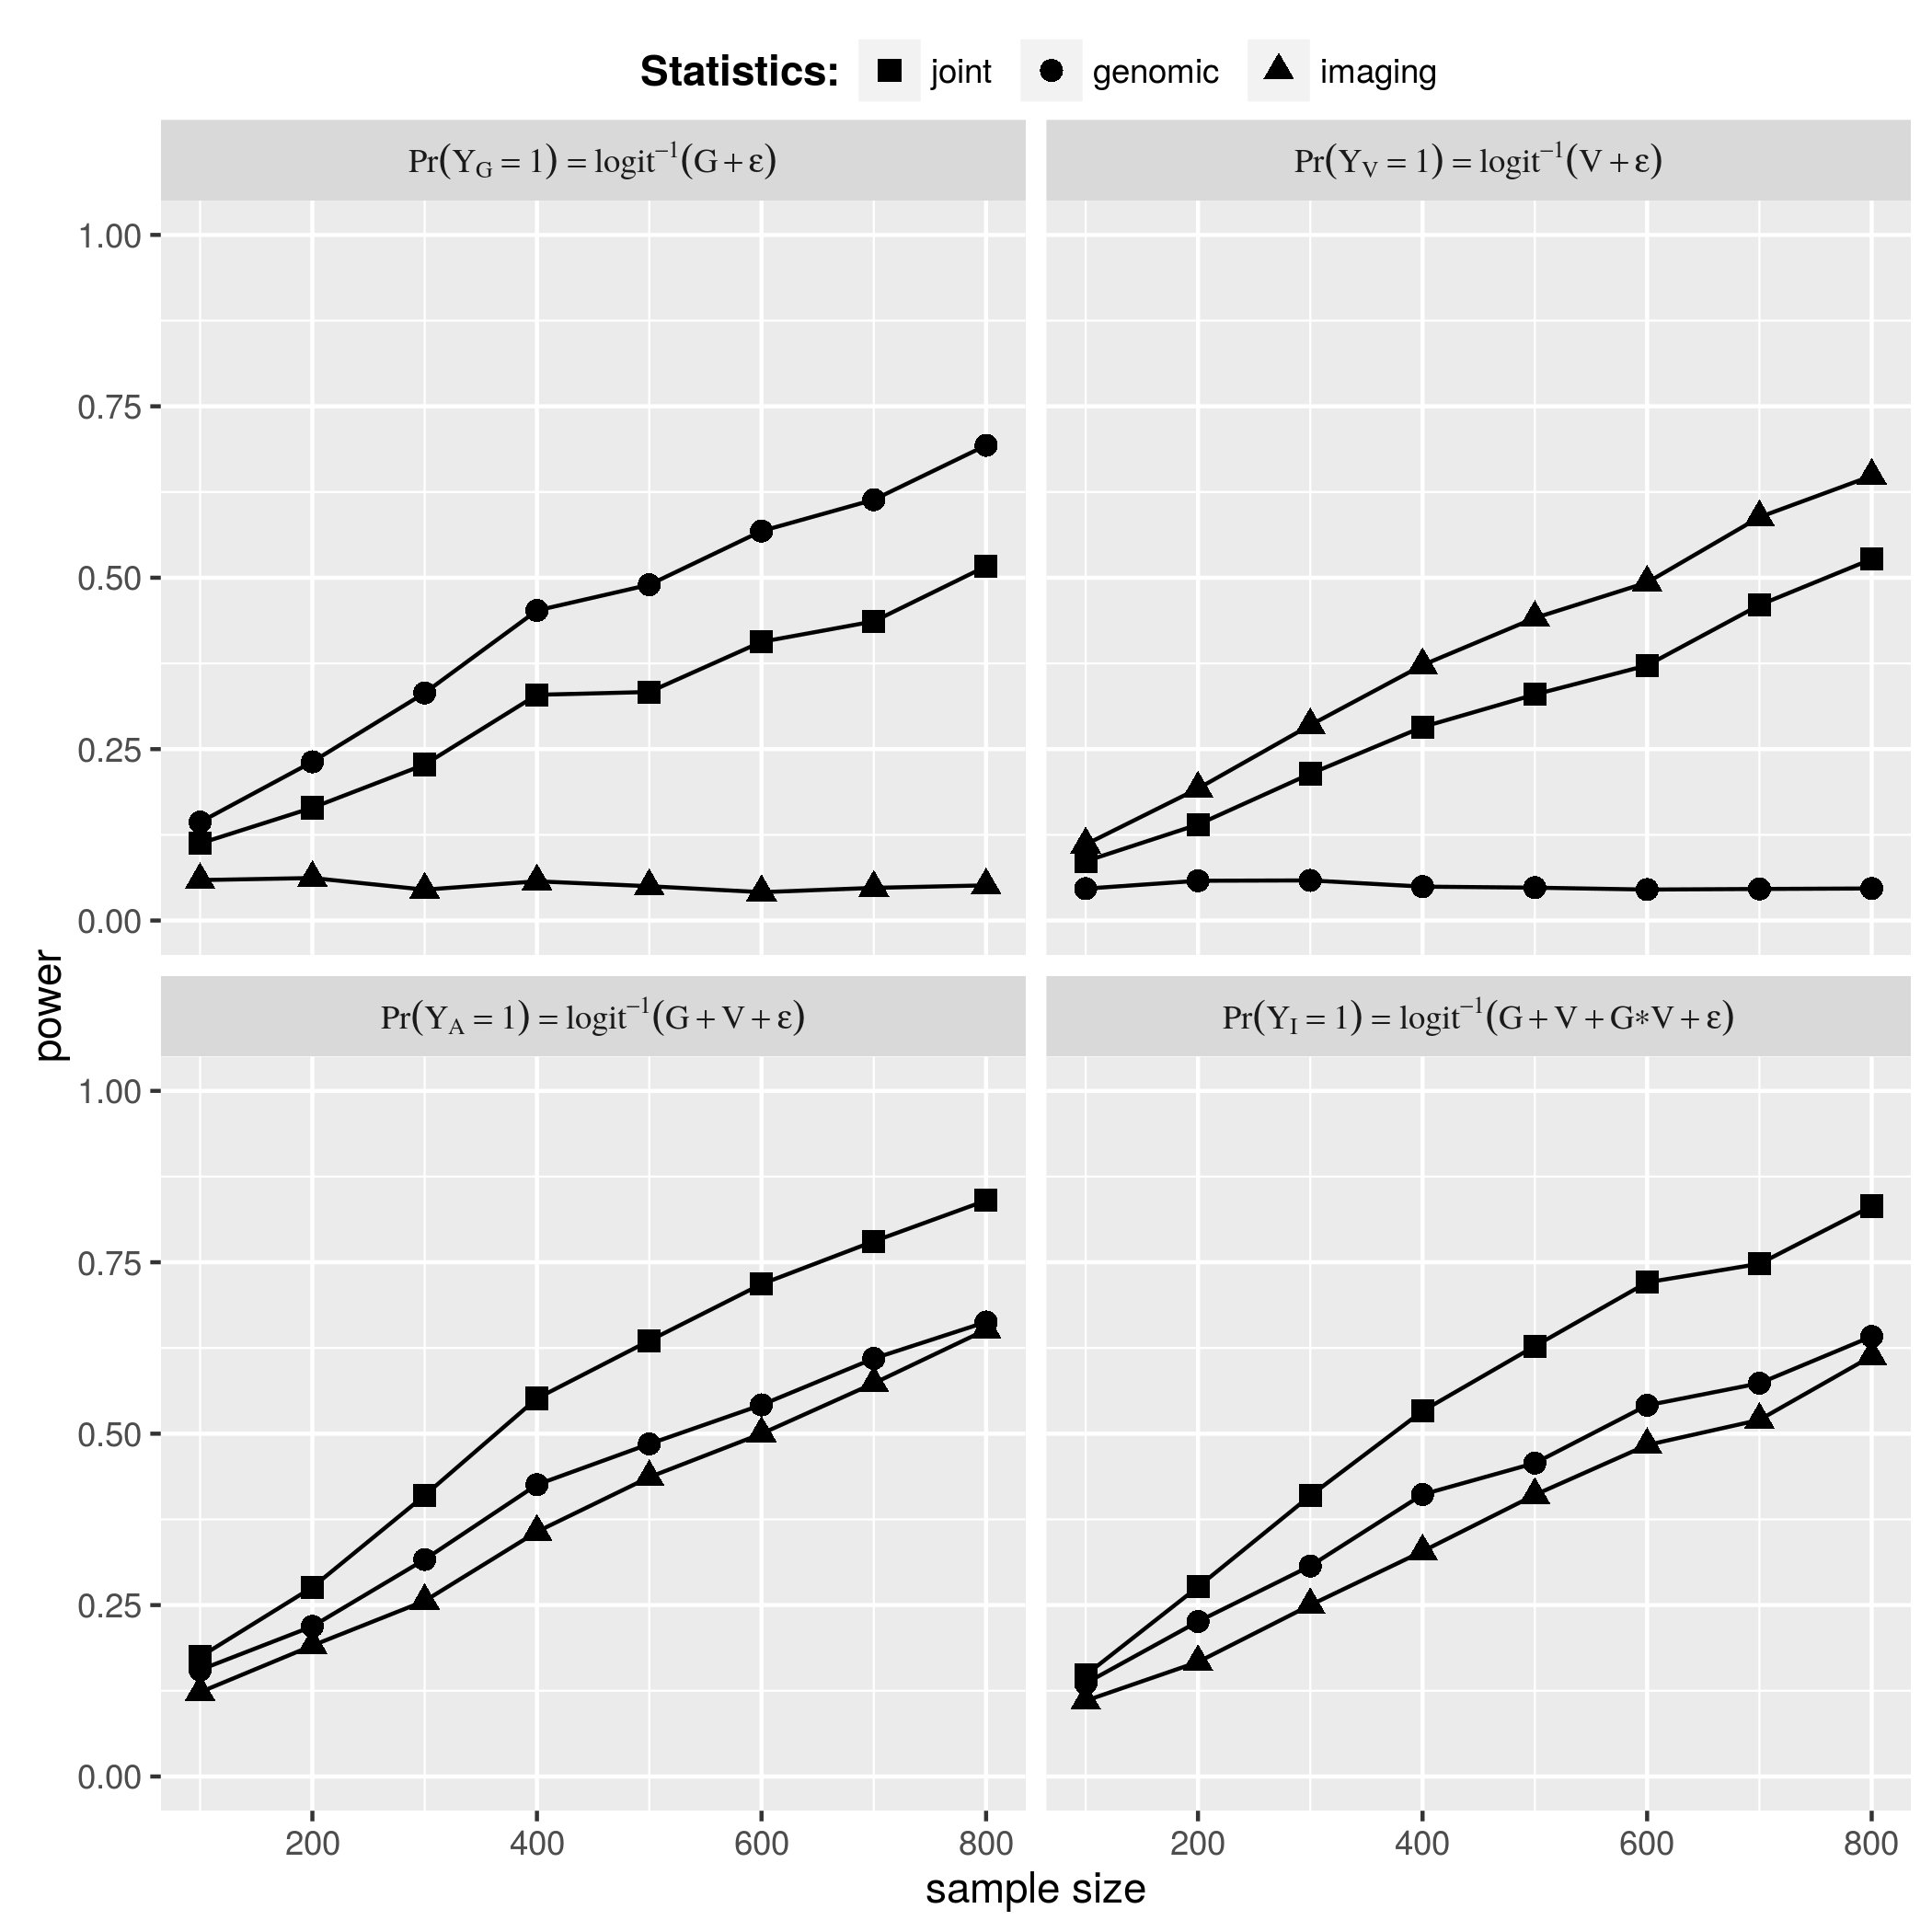
\includegraphics[width=300px]{img/PWR_BIN_KNL.png}
\caption{Joint U v.s. Parsimonious U statistics (Binary)}
\end{figure}

\begin{figure}[!htbp]
\label{fig:PWR_BIN_VWA}
\centering
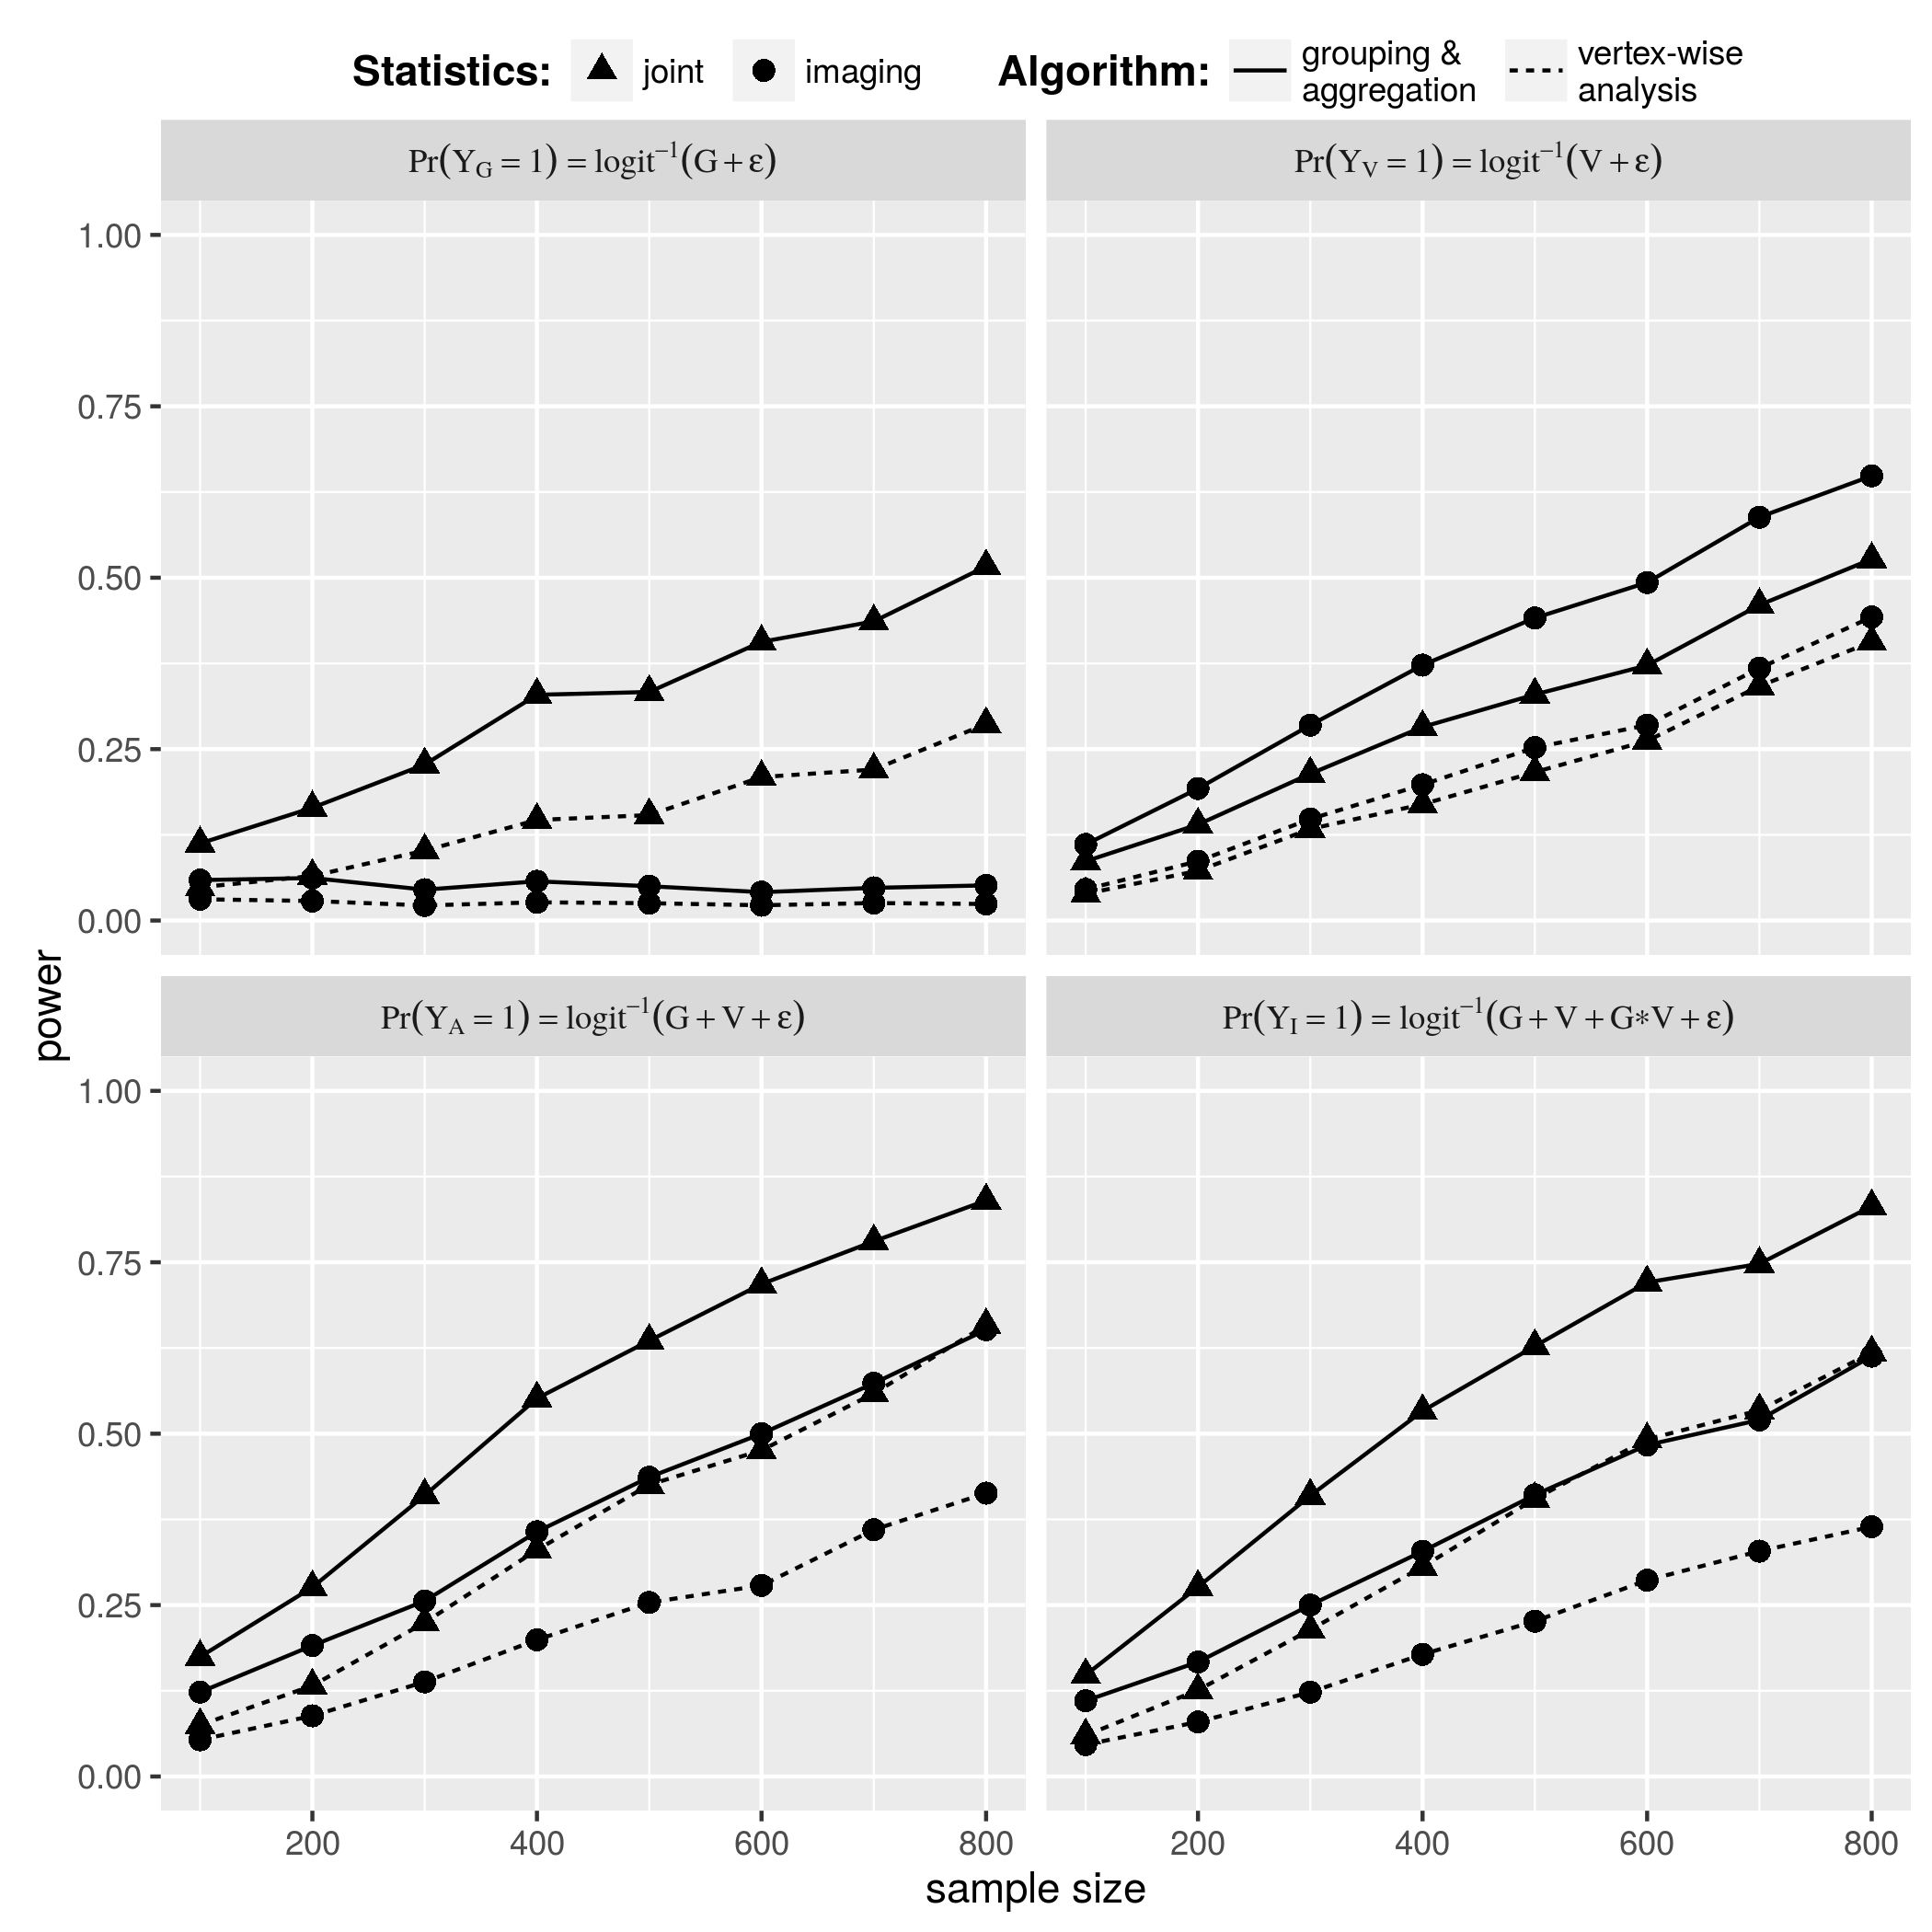
\includegraphics[width=300px]{img/PWR_BIN_VWA.png}
\caption{Vertex Grouping \& Aggregation v.s. Vertex-wise Analysis (Binary)}
\end{figure}

\begin{figure}[!htbp]
\label{fig:PWR_BIN_SAE}
\centering
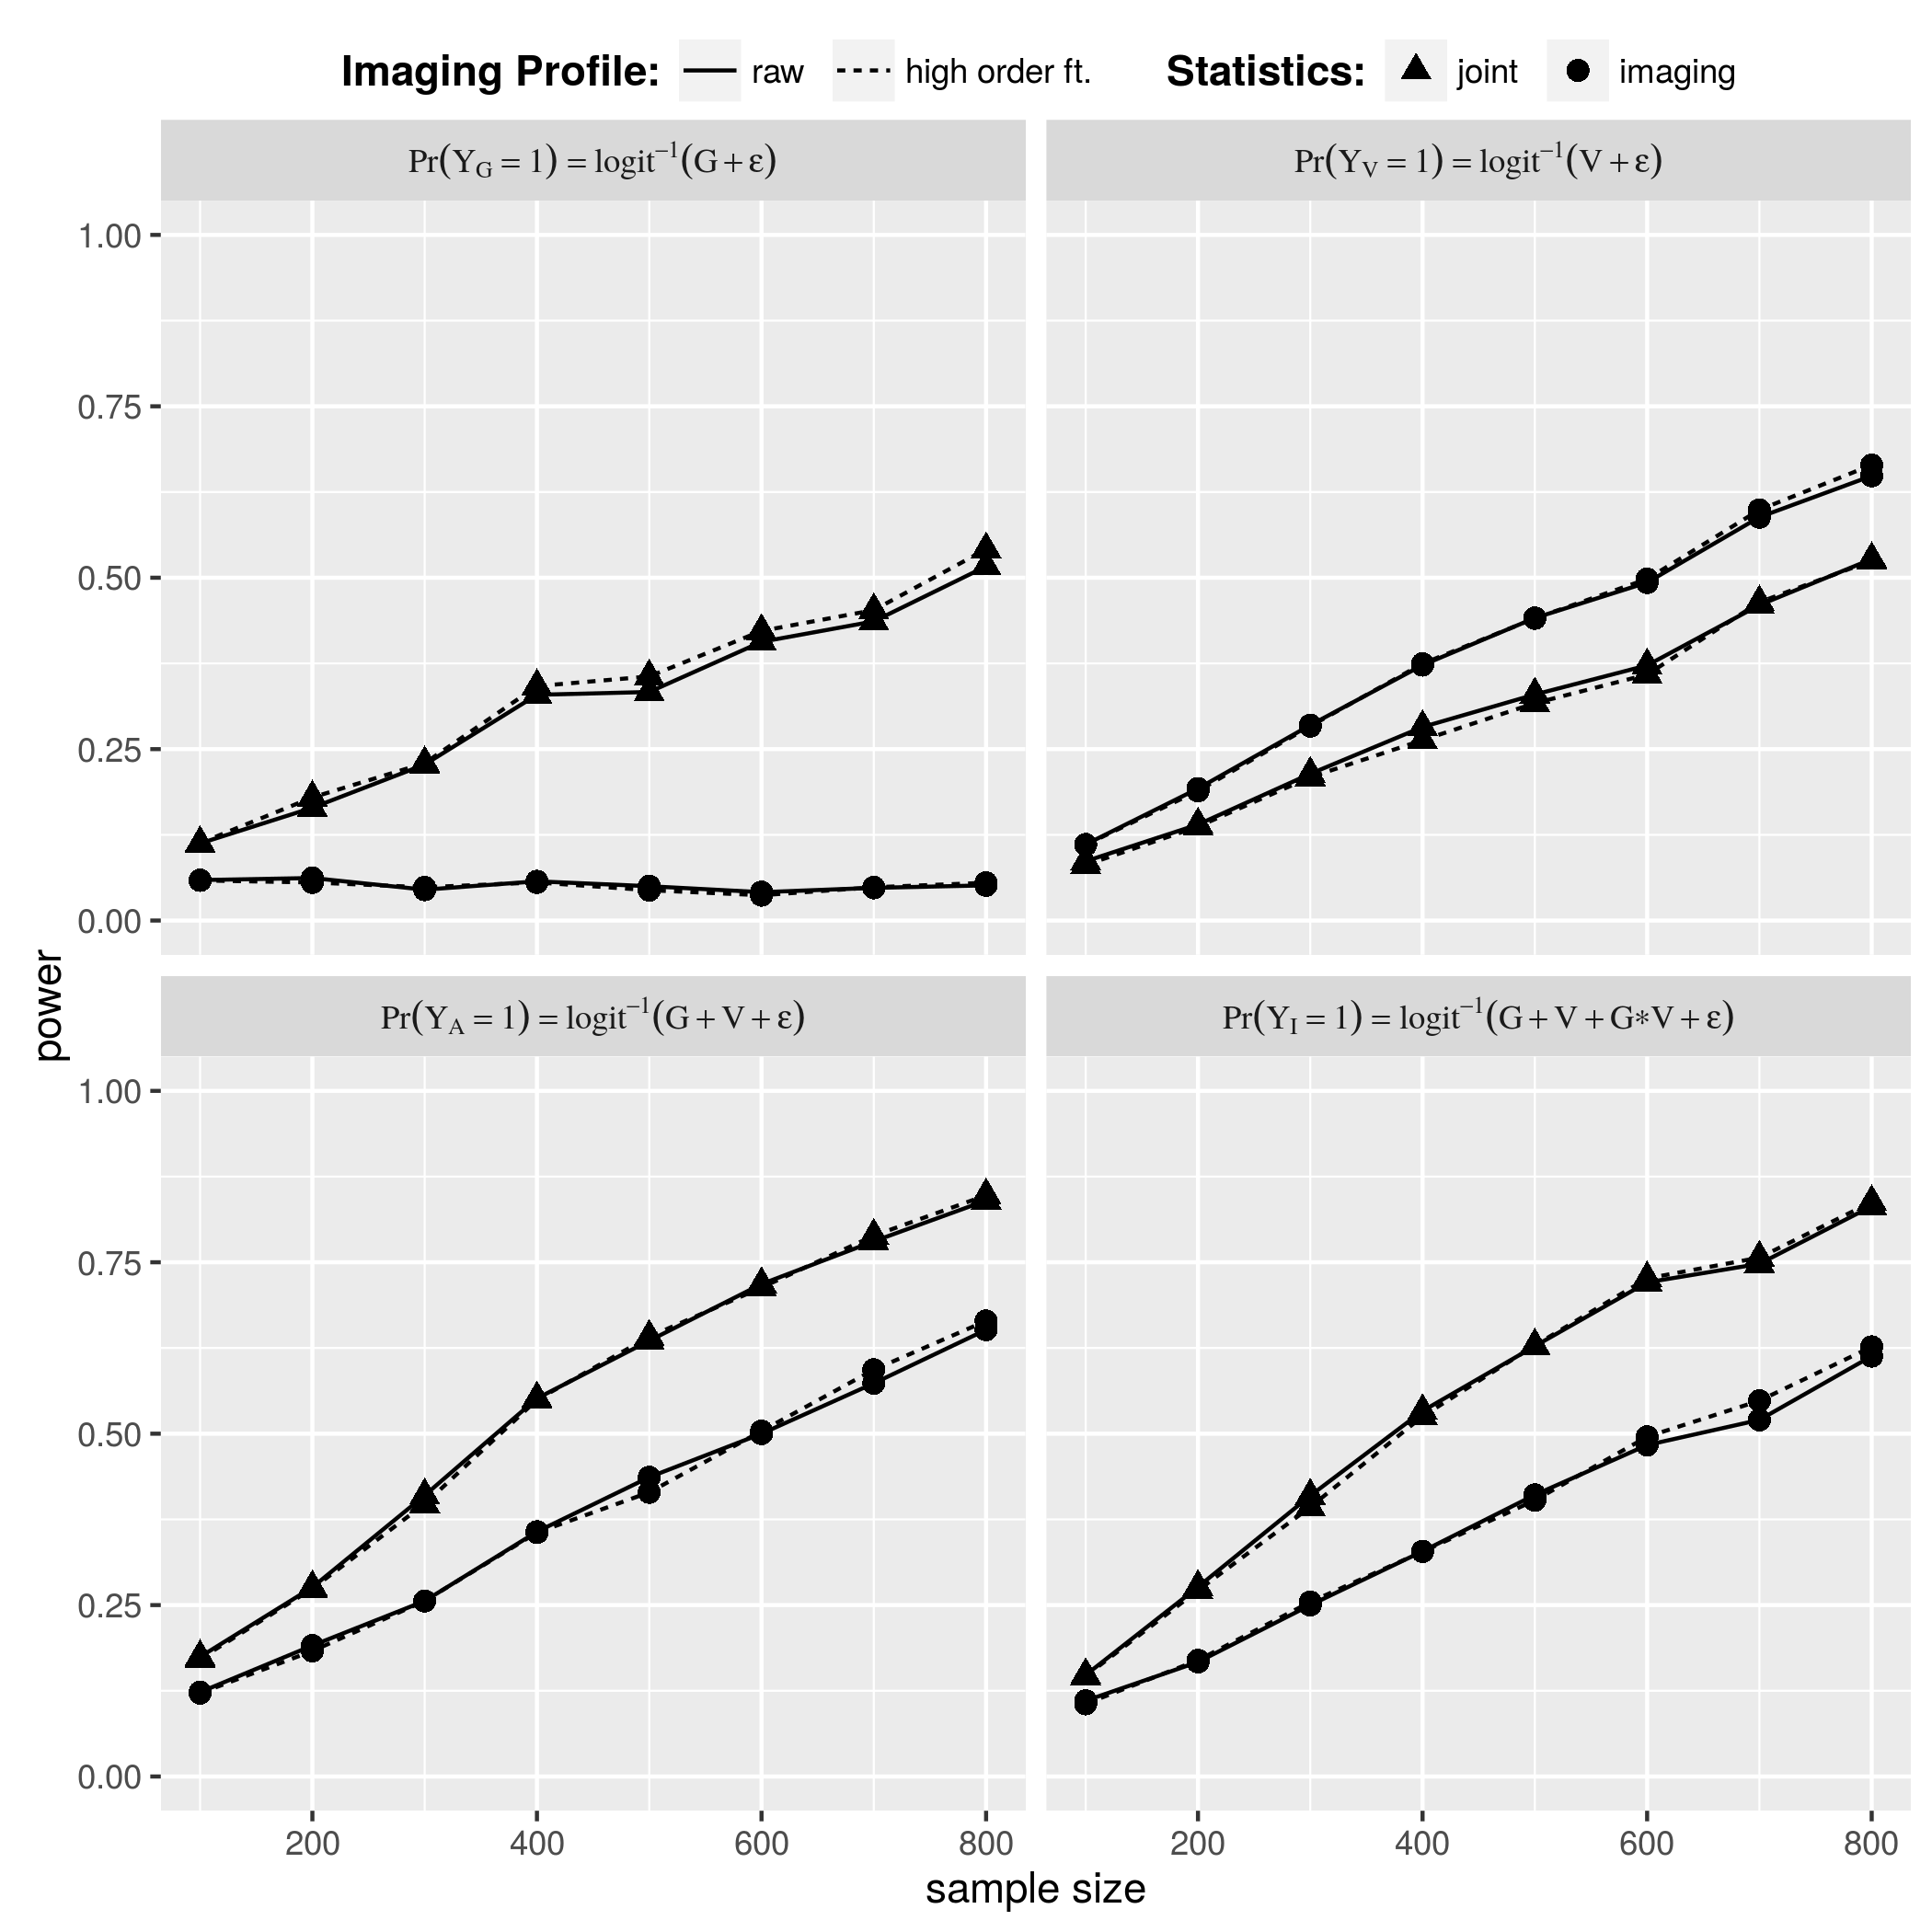
\includegraphics[width=300px]{img/PWR_BIN_SAE.png}
\caption{High order features v.s. original vertices}
\end{figure}

\end{document}
